\begin{figure}[htbp]
 \centering\leavevmode
 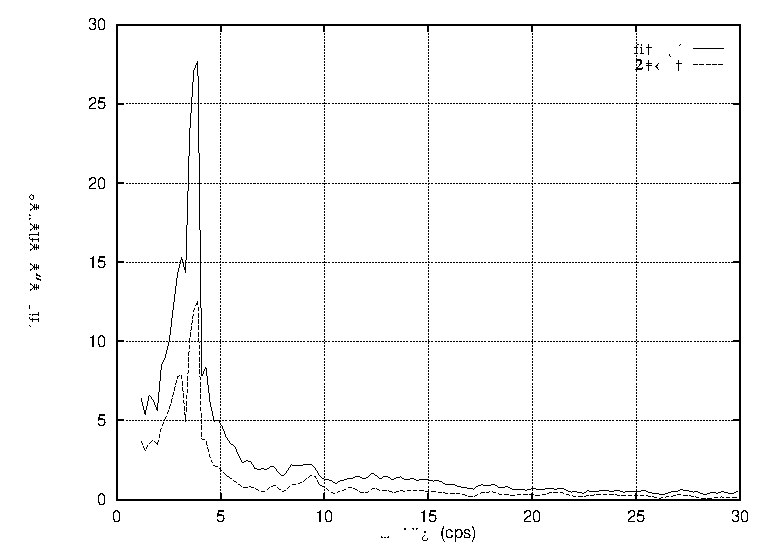
\includegraphics[height=0.4\textheight]{figs/FV/sh-b.ps}\label{sh-free}
 \caption{\$B<7>rE!(B $B<+M3?6F0%U!<%j%(%9%Z%/%H%k(B}
\end{figure}
\begin{figure}[htbp]
 \centering\leavevmode
 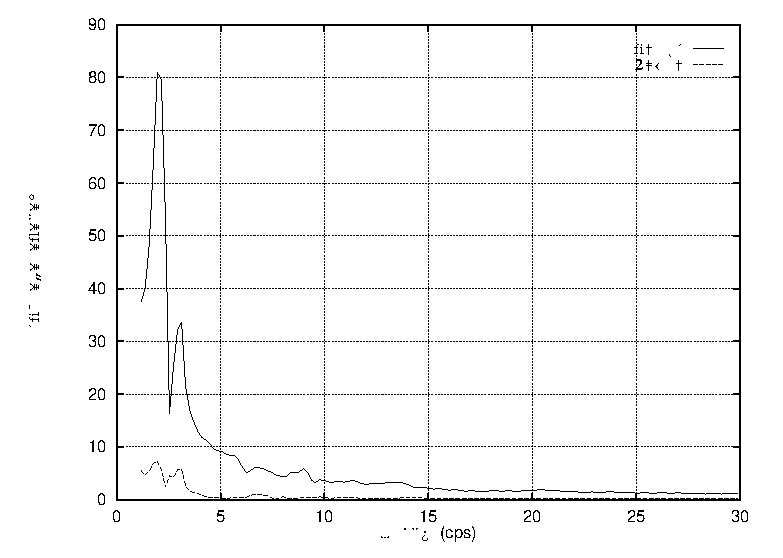
\includegraphics[height=0.4\textheight]{figs/FV/tu-a.ps}\label{tu-free}
 \caption{\$BDTE!(B $B<+M3?6F0%U!<%j%(%9%Z%/%H%k(B}
\end{figure}
\begin{figure}[htbp]
 \centering\leavevmode
 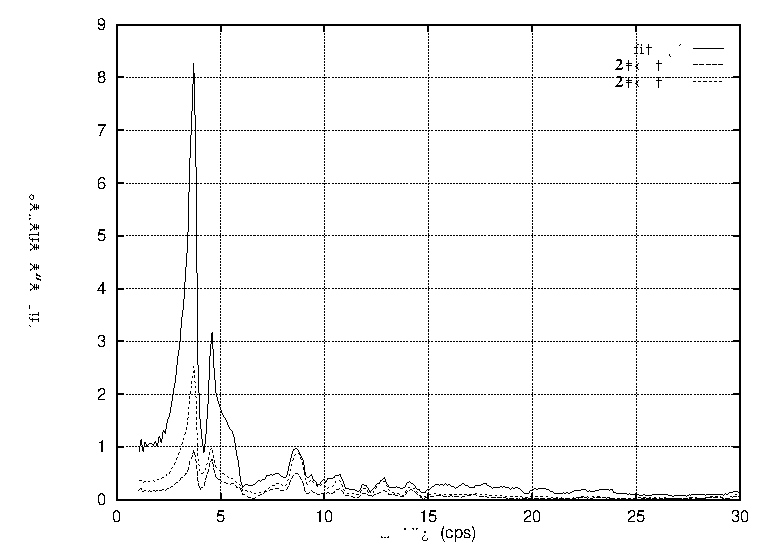
\includegraphics[height=0.4\textheight]{figs/FV/ta-f.ps}\label{ta-free}
 \caption{\$BEDCfE!(B $B<+M3?6F0%U!<%j%(%9%Z%/%H%k(B}
\end{figure}
\begin{figure}[htbp]
 \centering\leavevmode
 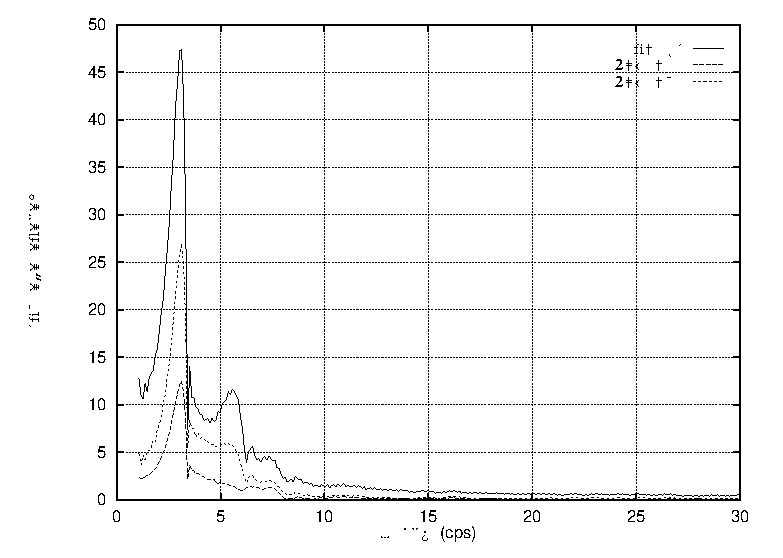
\includegraphics[height=0.4\textheight]{figs/FV/su-f.ps}\label{su-free}
 \caption{\$B?y1:E!(B $B<+M3?6F0%U!<%j%(%9%Z%/%H%k(B}
\end{figure}
\begin{figure}[htbp]
 \centering\leavevmode
 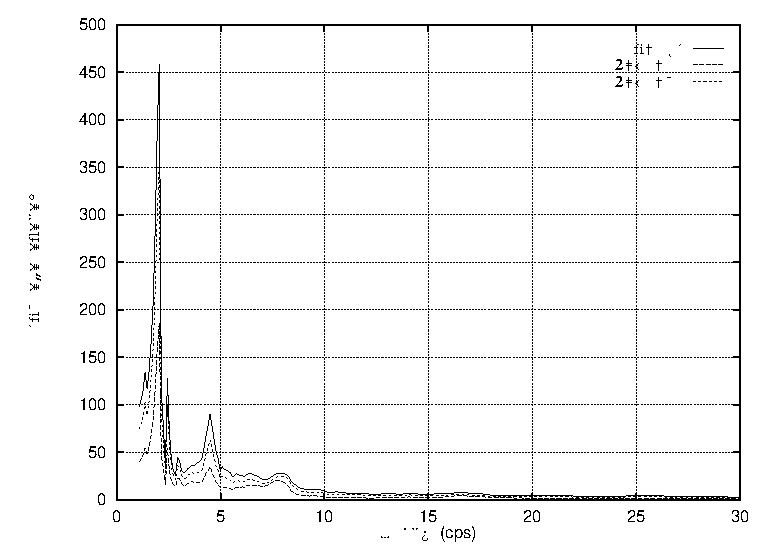
\includegraphics[height=0.4\textheight]{figs/FV/hau-f.ps}\label{hau-free}
 \caption{\$B%O%&%a%C%;(B $B<+M3?6F0%U!<%j%(%9%Z%/%H%k(B}
\end{figure}

%%% Local Variables: 
%%% mode: latex
%%% TeX-master: "paper"
%%% End: 
